%
% Copyright (c) 2001 LAAS/CNRS                        --  Thu Oct 18 2001
% All rights reserved.                                     Anthony Mallet
%
% This document is a translation of the French documentation of GenoM,
% originally written by Sara Fleury and Matthieu Herrb.
%
% Redistribution  and  use in source   and binary forms,  with or without
% modification, are permitted provided that  the following conditions are
% met:
%
%   1. Redistributions  of  source code must  retain  the above copyright
%      notice, this list of conditions and the following disclaimer.
%   2. Redistributions in binary form must  reproduce the above copyright
%      notice,  this list of  conditions and  the following disclaimer in
%      the  documentation   and/or  other  materials   provided with  the
%      distribution.
%
% THIS SOFTWARE IS PROVIDED BY THE  AUTHOR AND CONTRIBUTORS ``AS IS'' AND
% ANY  EXPRESS OR IMPLIED WARRANTIES, INCLUDING,  BUT NOT LIMITED TO, THE
% IMPLIED WARRANTIES   OF MERCHANTABILITY AND  FITNESS  FOR  A PARTICULAR
% PURPOSE ARE DISCLAIMED.  IN NO  EVENT SHALL THE AUTHOR OR  CONTRIBUTORS
% BE LIABLE FOR ANY DIRECT, INDIRECT,  INCIDENTAL, SPECIAL, EXEMPLARY, OR
% CONSEQUENTIAL DAMAGES (INCLUDING,  BUT  NOT LIMITED TO, PROCUREMENT  OF
% SUBSTITUTE  GOODS OR SERVICES;  LOSS   OF  USE,  DATA, OR PROFITS;   OR
% BUSINESS  INTERRUPTION) HOWEVER CAUSED AND  ON ANY THEORY OF LIABILITY,
% WHETHER IN CONTRACT, STRICT LIABILITY, OR TORT (INCLUDING NEGLIGENCE OR
% OTHERWISE) ARISING IN ANY WAY OUT OF THE  USE OF THIS SOFTWARE, EVEN IF
% ADVISED OF THE POSSIBILITY OF SUCH DAMAGE.
%
% $Id$
%

A module is described with a particular syntax  in a file whose name ends
in ``dot   gen'' ({\tt .gen}).  In this   chapter, we will  write  a test
module which we will call ``demo''.  Thus the file describing this module
will be  called  {\tt demo.gen}.  The next  sections  explain  how such a
module is generated and used.

% -----------------------------------------------------------------------
\section{Principle of the module generation}
\label{sec|session|principle}

One can distinguish two main parts in a module:

\begin{itemize}
   \item A {\em server}, which encapsulate algorithms and is generated
automatically by \GenoM\ from the description file,
   \item The set of {\em algorithms} that you have developed, and that
will be included into the module.
\end{itemize}

To combine these two parts and form  a complete module, the definition of
functions that  will interface the server and  the algorithms together is
required (at the moment  only {\tt  C}  functions are  supported).  These
functions are  called ``codels'' (which  stands for {\em code elements}),
and they represent the {\em smallest} grain size  the server will be able
to manipulate.

The first  time \GenoM\  is called,  it generates empty  codels. They are
fully  functional, but do  nothing. It's up to  you to fill  them in with
your own code.

\bigbreak

\begin{figure}[htbp]
\centering
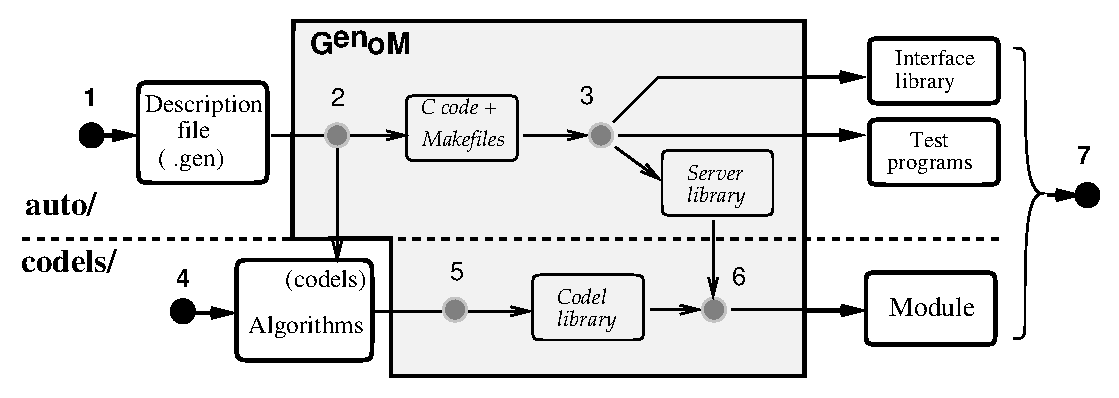
\includegraphics[width=0.8\hsize]{fig/cycle-en}
\caption{Development cycle and separation between sever and codels.}
\label{fig|session|cycle}
\end{figure}

To help   you distinguish  between   the  server   and the   codels,  the
corresponding files are placed in two separate directories. The first one
is called {\tt auto/} and contains all  the code generated by \GenoM. The
second directory is called {\tt   codels/} and  contains the codels   ---
initially a template generated by \GenoM\ but never touched again once
you have filled them in.

\bigbreak

The figure~\ref{fig|session|cycle} shows a synthetic view of the
separation between {\tt auto/} and {\tt codels/} and also represent a
typical development cycle~:

\begin{description}
   \item{\bf 1. module description:} edition of the {\tt .gen} file,
   \item{2. and 3. server generation and compilation},
   \item{\bf 4. write the codels that will invoke your algorithms},
   \item{5. and 6. compile the codels and link with the server},
   \item{\bf 7. test and use the module}.
\end{description}

Only the points {\bf 1}, {\bf 4} and {\bf  7} are in your charge. \GenoM\
writes for you   the {\tt Makefile}s  and  handle the compilation of  the
various files.

Once you have  compiled a module,  you  can incrementally modify, add  or
remove services (back to  the first point) and  codels (back to the point
number 4).

% -----------------------------------------------------------------------
\section{An example}
\label{sec|session|example}

This section will  illustrate a concrete use  of \GenoM\ with  a ``demo''
module. This module  will  control a  mobile that  can translate  on  a 2
meters long rail. Some of the services the ``demo'' module offers are:

\begin{itemize}
   \item select the speed (between two symbolic values {\tt DEMO\_SLOW}
and {\tt DEMO\_FAST}),
   \item move the mobile for a given distance,
   \item read the current speed or position at any moment,
   \item suspend the motion,
   \item monitor particular positions and inform when the mobile goes
through these positions.
\end{itemize}

To implement this, we first create a directory named {\tt demo/}. In that
directory we will write the description file {\tt demo.gen}, which could
look like this (see next page):
\vfill\eject

\vbox to\textheight{\vfill
\begin{center}
\begin{cartouche}\small
\begin{verbatim}
/* -------------------------- MODULE DECLARATION --------------------------- */

module demo {
   number:            9000;            /* module id: unique number */
   internal_data:     DEMO_STR;        /* C typedef (defined below) */
};


/* ------------- DEFINITION OF THE MODULE's INTERNAL DATABASE -------------- */

/* External definitions involved in the database definition */
#include "demoStruct.h"

/* The internal database */
typedef struct DEMO_STR {
   DEMO_STATE_STR   state;           /* Current state of the mobile */
                                     /* (position and speed) */
   DEMO_SPEED       speedRef;        /* Speed reference */
   double           distRef;         /* Distance reference */
   double           monitor;         /* Positions monitors */
}DEMO_STR;
 

/* ------------------ SERVICES DEFINITION: The REQUESTS -------------------- */

/* Control request: modify the default speed */
request SetSpeed {
   type:                control;              /* request's type  */
   input:               speed::speedRef;      /* input: speed chosen */
   c_control_func:      demoControlSpeed;     /* codel for validity checks */
   fail_msg:            INVALID_SPEED;        /* possible error messages */
};

/* Control request: return the default speed */
request GetSpeed {
   type:                control;              /* request's type */
   output:              speed::speedRef;      /* output: the speed */
};

/* Control request:  interrupt the mobile */
request Stop {
   type:                control;              /* request's type */
   incompatible_with:   MoveDistance;         /* request to interrupt */
};
\end{verbatim}
\end{cartouche}
\end{center}
\vfill
\hfill continued on next page...
}
\eject

\vbox to\textheight{
... continuation of previous page
\vfill
\begin{center}
\begin{cartouche}\small
\begin{verbatim}
/* Execution request: translate of a given distance */
request MoveDistance {
   type:                exec;                 /* request's type */
   input:               distance::distRef;    /* input: distance */
   c_control_func:      demoControlDistance;  /* codel for validity checks */
   fail_msg:            TOO_FAR_AWAY;         /* possible error messages */
   c_exec_func_start:   demoStartEngin;       /* initialization codel */
   c_exec_func:         demoGotoPosition;     /* main codel */
   c_exec_func_end:     demoStopEngin;        /* termination codel */
   c_exec_func_inter:   demoStopEngin;        /* interruption codel */
   incompatible_with:   MoveDistance;         /* incompatible requests */
   exec_task:           MotionTask;           /* task (thread) executing
                                               * the codel */
};

/* Execution request: monitor a particular mobile's position */
request Monitor {
   type:                exec;                 /* request's type */
   input:               position::monitor;    /* inputs: position */
   output:              position::state.position; /* outputs: actual pos. */
   c_exec_func:         demoMonitor;          /* main codel */
   fail_msg:            TOO_FAR_AWAY;         /* possible error messages */
   incompatible_with:   none;                 /* no incompatible requests */
   exec_task:           MotionTask;           /* task (thread) */
};


/* ------------------------ POSTERS DECLARATION  --------------------------- */

/* Poster that exports the current state of the mobile */
poster Mobile {
   update:               auto;
   data:                 state::state, ref::distRef;
   exec_task:            MotionTask;
};

 
/* --------------------- EXECUTION TASKS DECLARATION ----------------------- */

/* Only one task (or thread) */
exec_task MotionTask {
   period:               20;
   delay:                0;
   priority:             100;
   stack_size:           2000;
   c_init_func:          demoInit;
};
\end{verbatim}
\end{cartouche}
\end{center}
\vfill
}
\eject

The file {\tt demo.gen} is made up of five parts, each of them being
identified with a keyword (these keywords are explained in detail in
chapter \ref{cha|edit}):

\begin{center}\begin{tabular}{llll}
1.& {\tt module} & module declaration \\
\noalign{\vskip10pt}

2.& \parbox[t]{4cm}{
\hbox{\tt \#include} and
\hbox{\tt typedef struct}} & \parbox[t]{9cm}{{\tt C} include
statement for the definition of structures and declaration of the
internal database} \\
\noalign{\vskip10pt}

3.& {\tt request} & \parbox[t]{9cm}{requests definition: the five
services offered by the module} \\
\noalign{\vskip10pt}

4.&  {\tt   poster} & \parbox[t]{9cm}{posters  definition:   posters  are
exported  data structures  that let information  on the  mobile  state be
available for other modules} \\
\noalign{\vskip10pt}

5.& {\tt exec\_task} & \parbox[t]{9cm}{execution task declaration (a
thread for Unix) that take care of codel execution}\\
\end{tabular}\end{center}

\bigbreak

The {\tt \#include demoStruct.h} statement (the  second part above) works
as in {\tt C} and  includes the corresponding {\tt  C} header file.  This
file contains   all the necessary   {\tt  typedef} declarations  for  the
definition of the  internal database. These structures  are  then used by
the {\tt request} and the {\tt poster} declarations.

In this example,  the file {\tt  demoStruct.h} contains the definition of
{\tt  DEMO\_STATE\_STR} and  {\tt DEMO\_SPEED}. This   file is preferably
located in the same directory as {\tt demo.gen},  since it contributes to
the definition of the module interface.

\bigbreak

\begin{center}
\begin{cartouche}\small
\begin{verbatim}
#ifndef DEMO_STRUCT_H
#define DEMO_STRUCT_H

/* Current state of the mobile */
typedef struct DEMO_STATE_STR {
   double position;              /* current position */
   double speed;                 /* current speed */
}DEMO_STATE_STR;

/* Admissible speeds */
typedef enum DEMO_SPEED{
  DEMO_SLOW,                     /* low speed */
  DEMO_FAST                      /* high speed */
} DEMO_SPEED;

#endif /* DEMO_STRUCT_H */
\end{verbatim}
\end{cartouche}
\end{center}


% -----------------------------------------------------------------------
\section{Module generation}
\label{sec|session|generate}

The  generation step is done  through the {\tt genom} command invocation.
When a module is to be generated for the  first time, {\tt genom} must be
invoked  with the {\tt  -i} option, which installs  the initial files (in
particular, it installs the codels templates).  Here is a sample run, for
the {\tt demo} example:

\begin{center}
\begin{cartouche}\small
\begin{verbatim}
r2d2[demo] genom -i demo
Module Generator GenoM
Copyright (C) LAAS/CNRS 1994-1996
No directory auto, install it ? (y/n) y
Entering directory `auto'
perl demo.pl
Creating directory user
Makefile.vxworks created
Makefile.unix created
Makefile.protos created
Makefile created
demoType.h created
demoError.h created
...
demoPrintProto.h is created
prototype demoScan.c
demoScanProto.h is created
Creating directory codels
codels/ is installed, from now you can just call "gnumake"
Done.
\end{verbatim}
\end{cartouche}
\end{center}

\bigbreak

Some comments on this run:

\begin{enumerate}
   \item  The {\tt   .gen}  extension   needs   not  to be    explicitely
   given. \GenoM\ appends it automatically.

   \item With the {\tt -i} option, \GenoM\ asked for a confirmation:
\begin{verbatim}
No directory auto, install it ? (y/n)
\end{verbatim}

   This is the first and also the last time  \GenoM\ asks for it. This is
   also your  last chance to abort the  module generation. Answer {\tt n}
   if you did not want to invoke {\tt genom}.

   \item \GenoM\ creates two directories and a great number of files. You
   do not need to know them all, and they will be described later in this
   document (they are also described in the appendix \ref{anx|files}).
\end{enumerate}

{\bf From now on, the module is ready to  be compiled and run}, but let's
look at the result of the execution of {\tt genom}:

\begin{center}
\begin{cartouche}\small
\begin{verbatim}
r2d2[demo] ls
Makefile       codels/        demoStruct.h      demo_essay*
auto/          demo.gen       startDemo
\end{verbatim}
\end{cartouche}
\end{center}

\bigbreak
\GenoM\ created two new directories {\tt auto/} and {\tt codels/}, and three
new files {\tt Makefile}, {\tt demo\_essay} and {\tt startDemo}:

\begin{itemize}
   \item The {\tt auto/} directory  is entirely dedicated to \GenoM\ (and
   that is the only  such directory).  It contains  all the  {\em server}
   code (see figure \ref{fig|session|cycle}), and you do not need to look
   into it, except if you are looking for some specific information. This
   document will describe this directory later.

   \item Algorithms (or a part of them) are grouped in the directory {\tt
   codels/}. It has been  installed by the  {\tt -i} option. The files in
   that directory give you a template to start from, and also let \GenoM\
   produce a module even if you still do not have written a single line of
   code. From now  on,  that directory belongs to  you  and \GenoM\ never
   goes into it again (except if you regenerate  the module with the {\tt
   -i} option).

   \item The  {\tt Makefile} file is  also under your control. That's the
   main file which is used for the compilation of the module. By default,
   it lets you specify which target you want to compile  for, but you can
   modify it to suit your needs.

   \item The  file {\tt startDemo} is a  tiny script for VxWorks, and let
   you load your module and start it. It also belongs to you.

   \item The  file  {\tt demo\_essay}  is a Unix  script that   starts an
   interactive test program for this module.
\end{itemize}


% -----------------------------------------------------------------------
\section{Module compilation}
\label{sec|session|compile}

{\bf Attention:   This  description  of  the   compilation step  might be
deprecated at any time.}

The  compilation step is  very straightforward: first,  you must edit the
{\tt Makefile} in the {\tt demo} directory.  Select  the target hosts for
which you  want to build the module   (Unix, VxWorks/ppc or VxWorks/m68k)
and  modify the  {\tt  all} target accordingly. Then,   you  just need to
invoke GNUmake in the {\tt demo/} directory.

\begin{center}
\begin{cartouche}\small
\begin{verbatim}
r2d2[demo] gnumake
-- Generate module
Module Generator GenoM
Copyright (C) LAAS/CNRS 1994-1996
Your module is up to date.

-- SERVER unix: server and client
...
-- CODELS unix
...
\end{verbatim}
\end{cartouche}
\end{center}

We can notice  that the Makefile  invoked  \GenoM\ again. This  allows to
check if the module  is still up-to-date  (that's the case in the example
above).  If the  {\tt .gen} file  (or  a file on   which it depends) were
locally modified, the module would have been regenerated.

{\bf Consequently, you just have to call  GNUmake to either regenerate or
compile the module. It is not necessary to invoke ``manually'' \GenoM.}


% -----------------------------------------------------------------------
\section{Module execution}
\label{sec|session|exec}

Once the server and the codels are compiled and  the link edition between
them has been done,  the {\tt demo} module is  ready to be executed.  The
module is located in    the  directory {\tt  codels/\$\{TARGET\}}    (see
figure~\ref{fig|session|cycle}), where {\tt \$\{TARGET\} =
\$\{MACHTYPE\}-\{OSTYPE\}}. Under Unix, this is an executable whose name is
the   name   of the     module  (under  Solaris   this  would    be  {\tt
codels/sparc-solaris/demo})  and under  VxWorks   this is an object  file
(for instance  {\tt codels/m68k-vxworks/demo.o}).

The   next two sections   present a step-by-step   tutorial on how to run
modules under   Unix  (section~\ref{ssec|exec|unix}) or   VxWorks systems
(section~\ref{ssec|exec|vxworks}).

\subsection{Execution under Unix}
\label{ssec|exec|unix}

{\bf  Attention:  The description of  the execution   under Unix might be
obsoleted at any time.}

\paragraph{Module startup:}

\begin{enumerate}
\item Launch {\tt h2 init} to initialize communication libraries.

\begin{center}\begin{cartouche}\small\begin{verbatim}
r2d2[demo] h2 init
Initializing csLib devices: OK
Hilare2 execution environment version 1.0
Copyright (c) 1999 LAAS/CNRS
\end{verbatim}\end{cartouche}\end{center}

Note: if you get the following message, it is usually sufficient to
answer {\tt n}:

\begin{center}\begin{cartouche}\small\begin{verbatim}
r2d2[demo] h2 init
Initializing csLib devices: 
Cslib devices already exist on this machine.
Do you want to delete and recreate them (y/n) ?
\end{verbatim}\end{cartouche}\end{center}

\item Launch the module.

\begin{center}\begin{cartouche}\small\begin{verbatim}
r2d2[demo] ./codels/sparc-solaris/demo -b
DEMO :
Spawn control task ... OK
Spawn task demoMotionTask ... OK
demo: All tasks are spawned
\end{verbatim}\end{cartouche}\end{center}

Note:  adapt  the path  to your system   (e.g. {\tt  i386/NetBSD} or {\tt
i386-linux}).

\item You're done! So... what?
\end{enumerate}

So the module is running and ready to serve requests. We will see how
this can be done with the small interactive test program {\tt demoEssay}
generated by \GenoM\ in the directory {\tt auto/\$\{TARGET\}}.

\paragraph{Client startup: the interactive test program {\tt demoEssay}}

This client can be launched with the shell script {\tt demo\_essay} in the
main directory of the module.

\begin{description} % for alignment
\item ~
\begin{center}\begin{cartouche}\small\begin{verbatim}
r2d2[demo] ./demo_essay 1
\end{verbatim}\end{cartouche}\end{center}
\end{description}

Note: if  you launch several clients, remember  to  change the number (we
choose ``1'' in the example above).

\paragraph{Killing the module:}

\begin{description} % for alignment
\item ~
\begin{center}\begin{cartouche}\small\begin{verbatim}
r2d2[demo] killmodule demo
\end{verbatim}\end{cartouche}\end{center}
\end{description}

At this point you can start a new instance of the module.

\paragraph{Cleaning everything:}

\begin{description} % for alignment
\item ~
\begin{center}\begin{cartouche}\small\begin{verbatim}
r2d2[demo] h2 end
\end{verbatim}\end{cartouche}\end{center}
\end{description}

\subsection{Execution under VxWorks}
\label{ssec|exec|vxworks}

\paragraph{Module startup:}

\begin{enumerate}
\item Log on the rack, using e.g. {\tt rlogin}
\item Change to the module directory

\begin{center}\begin{cartouche}\small\begin{verbatim}
cthulhu-> cd "/hilare2/src/modules/demo"
value = 0 = 0x0
\end{verbatim}\end{cartouche}\end{center}

Note: check the returned   value is '0'.  If  not, this is an  error (you
probably misspelled the directory name).

\item Load the module with {\tt ld}

\begin{center}\begin{cartouche}\small\begin{verbatim}
cthulhu-> ld < codels/m68k-vxworks/demo.o
value = 3436488 = 0x346fc8 = _semdemoInitExecTab + 0x12c
\end{verbatim}\end{cartouche}\end{center}

Note: adapt the path to your system (e.g. {\tt ppc-vxworks}).

\item Launch the module

\begin{center}\begin{cartouche}\small\begin{verbatim}
cthulhu-> demoTaskInit
DEMO :
Spawn control task ... OK
Spawn task demoMotionTask ... OK
demo: All tasks are spawned
value = 0 = 0x0
\end{verbatim}\end{cartouche}\end{center}

\item The module is running!
\end{enumerate}

The module is ready to serve  requests. We will see  how this can be done
with the small  interactive   test program {\tt demoEssay}   generated by
\GenoM\ in the directory {\tt auto/\$\{TARGET\}}.

\paragraph{Client startup: the interactive test program {\tt demoEssay}}

\begin{enumerate}

\item On the rack ({\em not} necessarily on the same CPU), you have to
load the module's {\em client library}. This library can send requests
to and receive answers from the module. It also contains the test
program.

\begin{center}\begin{cartouche}\small\begin{verbatim}
cthulhu-> ld < auto/m68k-vxworks/demoClient.o
value = 1289384 = 0x13aca8
\end{verbatim}\end{cartouche}\end{center}

\item Before you start the test program, you have to start on the remote
station  the utility {\tt xes\_server}   that let you  create terminals on
your local station from VxWorks. Check your DISPLAY environment variable
is correctly defined and do

\begin{center}\begin{cartouche}\small\begin{verbatim}
pif[] xes_server
xes_server version 2.3
Copyright (C) LAAS/CNRS 1992,1994
\end{verbatim}\end{cartouche}\end{center}

\item On the CPU where you loaded the client library, you can now
tell VxWorks  where your   {\tt xes\_server} lives   ({\tt pif}  in  this
example).

\begin{center}\begin{cartouche}\small\begin{verbatim}
cthulhu-> xes_set_host "pif"
value = 0 = 0x0
\end{verbatim}\end{cartouche}\end{center}

\item Last, launch the test program with the {\tt sp} command, with a
numeric argument between 0 and 9 indicating the instance number of this
client. 

\begin{center}\begin{cartouche}\small\begin{verbatim}
cthulhu-> sp demoEssay, 1
task spawned: id = 0x1335d0, name = t1
value = 1258960 = 0x1335d0
\end{verbatim}\end{cartouche}\end{center}

\end{enumerate}

If everything went well, a new terminal with a text  menu appears on your
screen.  Each request you  can send is associated  with a number, and you
can notice that the five  first commands (from  0 to 4) correspond to the
requests you defined  in  the file  {\tt  demo.gen}. The special  command
labeled '-99' let you kill the module.

A  detailed   description   of this interface   can    be  found   in the
section~\ref{sec|essay}, page~\pageref{sec|essay}.